\section{Experiments and Results}
\subsection{Experiment Setup}

For the main quantitative comparison, all strategies are tested on the same controlled random graph settings, task sequences, vehicle configurations, and evaluation metrics. The experiments focus on three questions: which fixed heuristic is the most stable baseline, whether Q-learning can learn useful rule-selection policies, and how charging-station selection affects scheduling performance.

\subsubsection{Environment Setup}
The environment is built on a graph-based road network with dynamic tasks, limited vehicles, battery constraints, load constraints, charging stations, and task deadlines. We test three scenario scales:
\begin{itemize}
    \item \textbf{Small:} 5 vehicles, 30 dynamic tasks, 2 charging stations, 25 road nodes, map size \(30\times 30\), and simulation horizon 180.
    \item \textbf{Medium:} 10 vehicles, 100 dynamic tasks, 4 charging stations, 60 road nodes, map size \(50\times 50\), and simulation horizon 300.
    \item \textbf{Large:} 20 vehicles, 300 dynamic tasks, 8 charging stations, 120 road nodes, map size \(80\times 80\), and simulation horizon 480.
\end{itemize}
We also compare two charging-station selection rules: \texttt{optimal\_station}, which considers both distance and station load, and \texttt{nearest\_station}, which always selects the nearest station.

\subsubsection{Evaluation Metrics}
We report task effectiveness, operating cost, and learning-stage metrics. Task effectiveness is measured by completed tasks, expired tasks, and final score. Operating cost is measured by total distance, simulation steps, makespan for offline planning, and charging burden. For Q-learning, we additionally report total training reward and evaluation score mean, which reflects the performance of the greedy policy after training.

\subsection{Experiment Results}

\subsubsection{Baseline Comparison}
\begin{figure}[htbp]
    \centering
    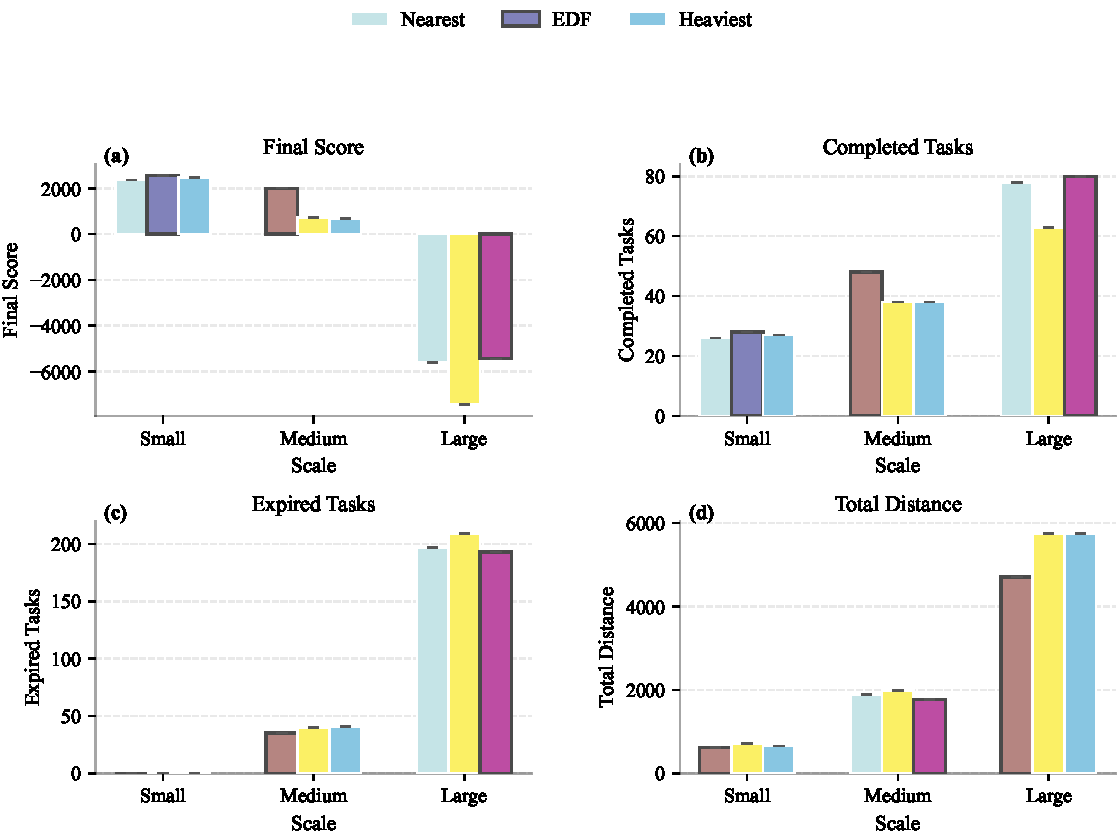
\includegraphics[width=\linewidth]{../experiments/figures/main/fig_baseline_multi_scale.pdf}
    \caption{Main comparison of heuristic baselines across three problem scales.}
    \label{fig:baseline_multi_scale}
\end{figure}

Figure~\ref{fig:baseline_multi_scale} compares Nearest, EDF, and Heaviest under different scenario scales. Since the total number of tasks differs across scales, completed tasks should be interpreted together with final score, expired tasks, and travel distance.

On the small scenario, the three heuristics are almost tied. Nearest obtains the highest average final score of \textbf{2354.10}, with \textbf{26.0} completed tasks and \textbf{0.4} expired tasks. EDF and Heaviest follow with scores of \textbf{2309.03} and \textbf{2271.05}. The gap is small because the task pressure is low and most vehicles can still find feasible tasks quickly.

The medium scenario separates the methods more clearly. Nearest remains the strongest baseline, with a final score of \textbf{3662.73}, \textbf{47.6} completed tasks, and \textbf{36.6} expired tasks. Heaviest ranks second, while EDF produces the weakest result among the three. A likely reason is that EDF focuses only on urgency and may send vehicles to distant tasks, which increases travel cost, battery consumption, and later deadline risk.

The large scenario is the most difficult one. All fixed rules suffer from more expired tasks, but Nearest still achieves the best score among fixed heuristics, followed by Heaviest and EDF. This suggests that distance-aware dispatching is a strong baseline in our simulator: shorter paths reduce energy consumption and leave more time for later tasks.

\subsubsection{Comparison with Q-learning}
\begin{figure}[htbp]
    \centering
    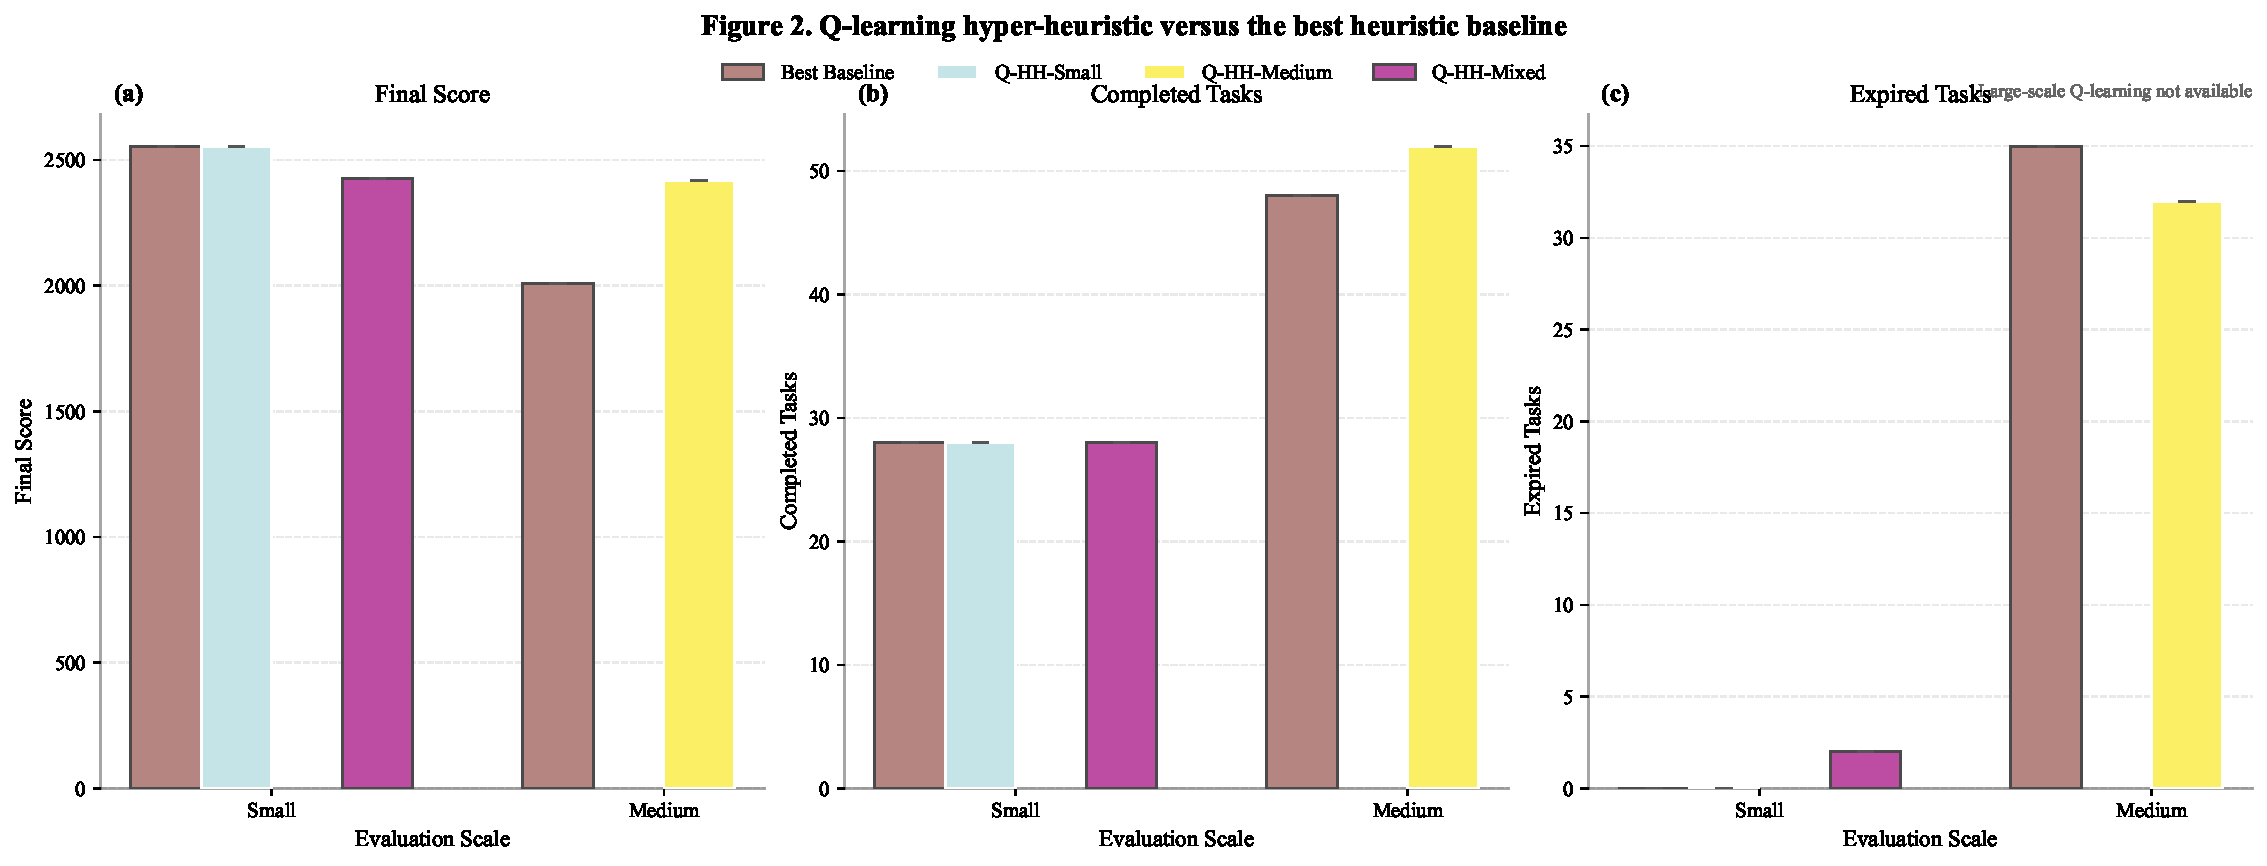
\includegraphics[width=0.8\linewidth]{../experiments/figures/main/fig_qlearning_vs_best_baseline.pdf}
    \caption{Overall comparison between Q-learning and the best baseline.}
    \label{fig:qlearning_vs_baseline}
\end{figure}

Figure~\ref{fig:qlearning_vs_baseline} compares the Q-learning hyper-heuristic with the strongest fixed baseline. In this experiment, Q-learning is evaluated as a rule-selection policy: it does not directly generate routes, but selects a low-level dispatching rule according to the current system state.

On small-scale evaluation, Q-HH-Small achieves a final score of \textbf{2399.09}, slightly higher than the best fixed baseline, while maintaining a similar task completion level. Q-HH-Mixed obtains a higher final score of \textbf{2515.96} and completes \textbf{28.2} tasks on average, but it also increases expired tasks to \textbf{1.8}. This suggests that mixed-scale training can improve task completion and score, but may also introduce more aggressive dispatching behavior.

In the medium-scale evaluation, Q-HH-Medium obtains a final score of \textbf{3050.90}, with \textbf{42.6} completed tasks and \textbf{43.6} expired tasks. This is lower than the Nearest baseline under the same scale. Therefore, the current tabular Q-learning policy is not consistently better than a strong fixed heuristic in more complex environments. The result is reasonable because medium-scale scenarios have denser task arrivals, larger state variation, and stronger coupling between task dispatching and charging decisions.

The training logs still show that Q-HH-Medium once reaches a best evaluation score of \textbf{4651.62}. This means Q-learning can discover high-quality rule-selection behavior, but the learned policy is not stable enough across evaluation seeds. Therefore, Q-learning is better viewed as a promising adaptive strategy rather than a fully dominant method in the current implementation.

\subsubsection{Training Convergence}
\begin{figure}[htbp]
    \centering
    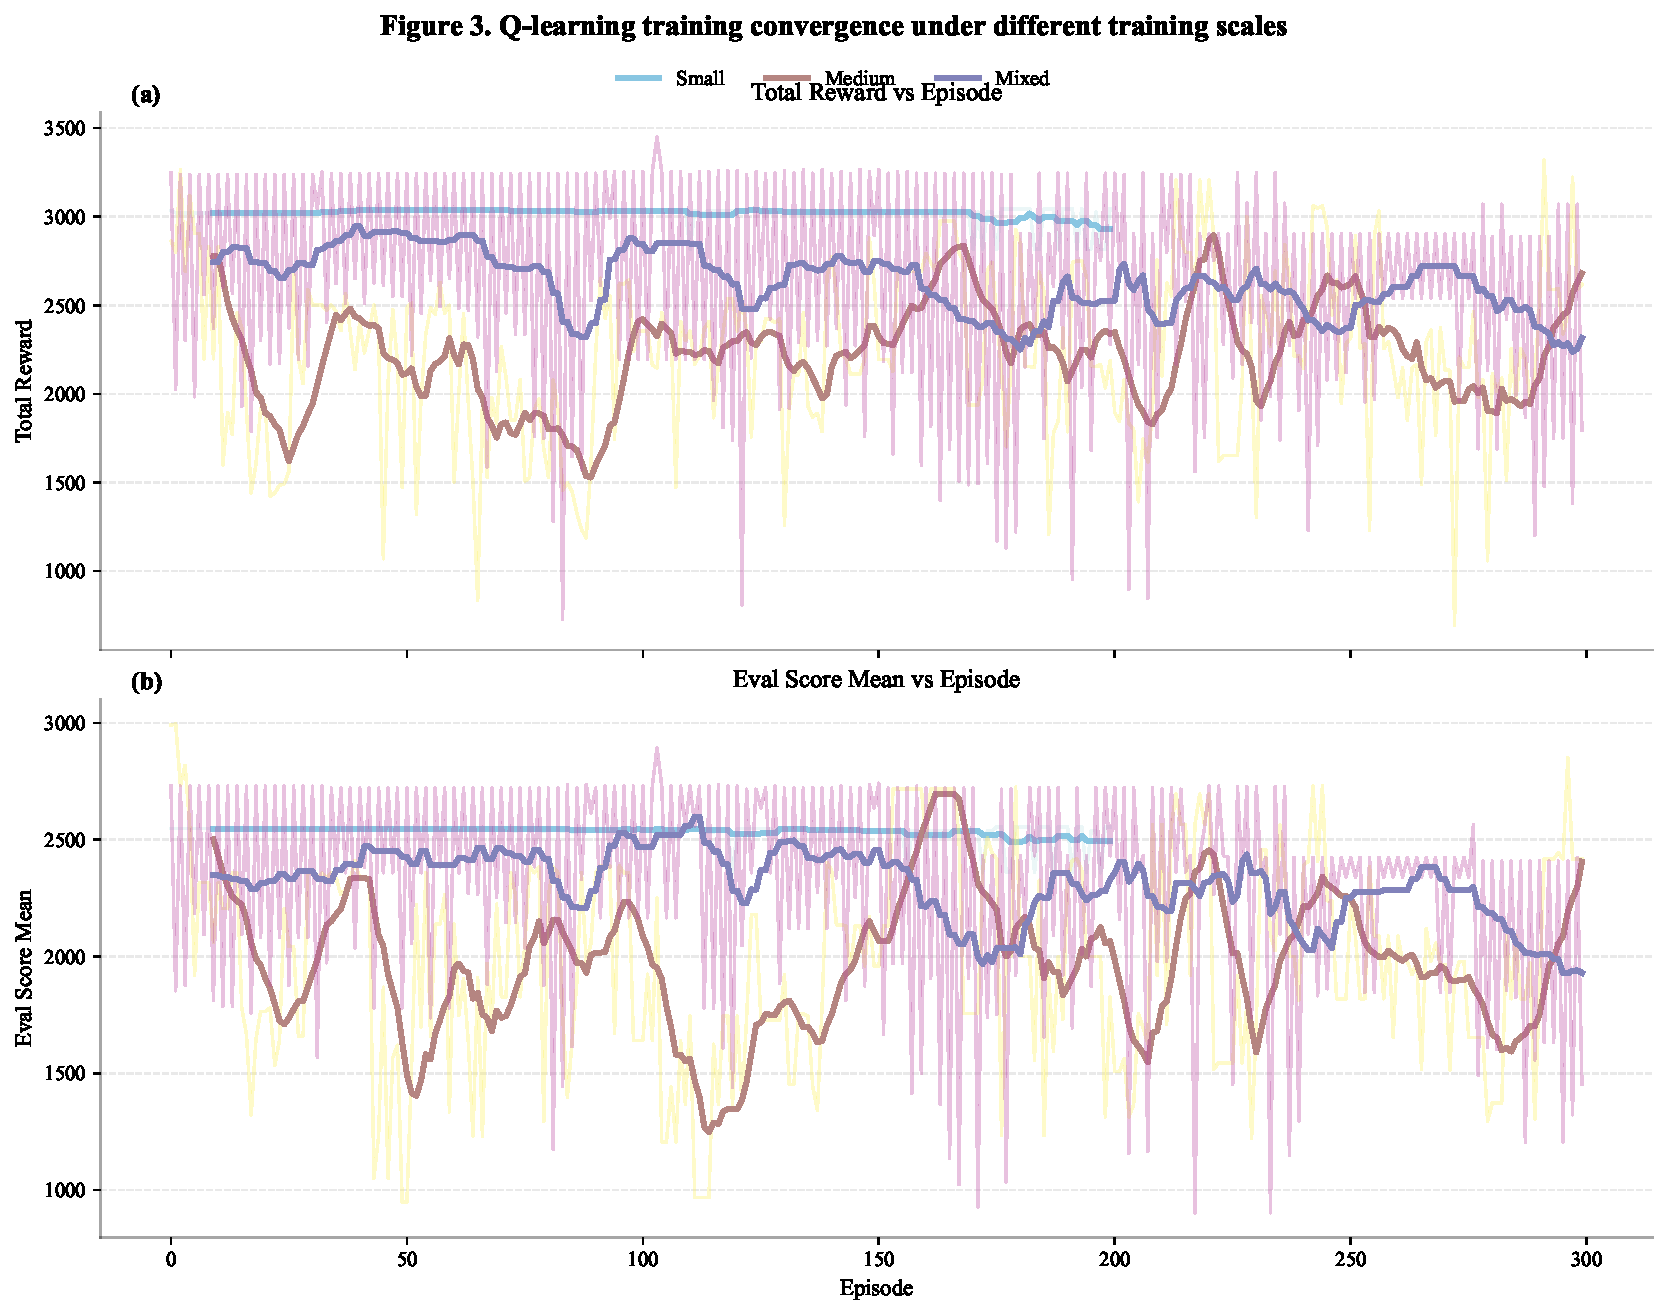
\includegraphics[width=\linewidth]{../experiments/figures/main/fig_qlearning_training_curves.pdf}
    \caption{Convergence curves of Q-learning under different training scales.}
    \label{fig:qlearning_convergence}
\end{figure}

Figure~\ref{fig:qlearning_convergence} shows that Q-learning improves policy quality during training, but its stability depends on scenario scale. The small-scale model is the most stable and reaches a best evaluation score of \textbf{2550.60} at episode \textbf{155}. The medium model reaches a higher best score of \textbf{4651.62} at episode \textbf{230}, but later evaluation performance decreases. The mixed-scale model also reaches a strong best score of \textbf{4455.95}, while its smoothed performance fluctuates because the training distribution alternates across different scales.

These results indicate that tabular Q-learning is feasible for adaptive rule selection, but its coarse state representation limits generalization in larger scenarios. Future work can improve this part by using richer state features, function approximation, or deep reinforcement learning methods such as DQN or PPO.

\subsubsection{Charging Strategy Ablation}
\begin{table}[htbp]
    \centering
    \caption{Charging strategy ablation results on the medium-scale setting.}
    \label{tab:charging_strategy_ablation}
    \resizebox{\linewidth}{!}{%
    \begin{tabular}{lrrrr}
        \toprule
        Method / strategy & Final Score & Completed & Expired & Avg. Queue \\
        \midrule
        Fixed baseline + optimal station & -- & \textbf{47.6} & \textbf{36.6} & \textbf{0.018} \\
        Fixed baseline + nearest station & -- & \textbf{47.6} & \textbf{36.6} & \textbf{0.018} \\
        Q-learning + optimal station & \textbf{2935.14} & \textbf{34.6} & \textbf{11.8} & -- \\
        Q-learning + nearest station & \textbf{2836.04} & \textbf{33.6} & \textbf{12.0} & -- \\
        \bottomrule
    \end{tabular}%
    }
\end{table}

Table~\ref{tab:charging_strategy_ablation} compares \texttt{optimal\_station} and \texttt{nearest\_station} in the medium-scale setting. For the fixed Nearest scheduler, the two charging strategies produce almost identical results: both complete \textbf{47.6} tasks, produce \textbf{36.6} expired tasks, and have an average queue load of only \textbf{0.018}. This suggests that charging congestion is not the main bottleneck in the current fixed-baseline runs.

For Q-learning, optimal station selection performs slightly better than nearest station selection. It obtains a final score of \textbf{2935.14}, compared with \textbf{2836.04} under nearest station selection. It also completes slightly more tasks and produces fewer expired tasks. This shows that charging decisions can interact with adaptive scheduling policies, although the effect is still limited under the current queue-load setting.

The experiments lead to three main findings. First, Nearest is a strong fixed baseline because it reduces both travel cost and energy risk. Second, Q-learning can learn useful rule-selection policies, but the current tabular version is not stable enough in medium-scale scenarios. Third, charging strategy design matters more when it interacts with adaptive scheduling, while its effect is small when station queues are light.
